\documentclass[border=4pt]{standalone}
\usepackage{amsmath,amssymb,tikz}\usetikzlibrary{arrows.meta}
\definecolor{figB}{RGB}{31,90,166}\definecolor{figR}{RGB}{176,48,48}\definecolor{figG}{RGB}{46,125,50}\definecolor{figO}{RGB}{214,120,20}
% T = 2 f1 e1^t + 0.8 f2 e2^t, e1 at 30 deg, f1 at 70 deg (same T as the SVD figure);
% matrix (0.968 -0.309 ; 1.491 1.177), det = 1.6
\begin{document}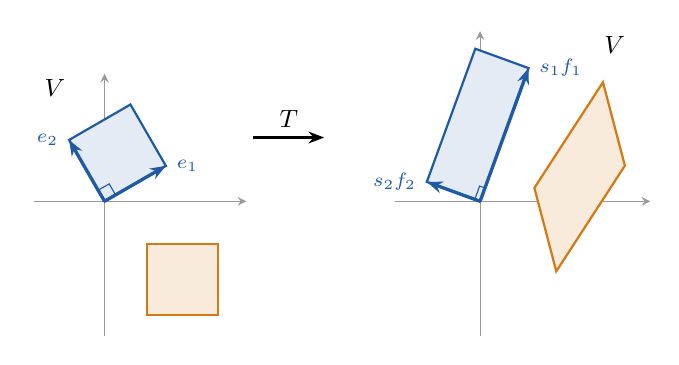
\begin{tikzpicture}[scale=0.9,>={Stealth[length=2mm]}]
\begin{scope}
\draw[black!40,thin,-stealth] (-1.0,0)--(2.0,0); \draw[black!40,thin,-stealth] (0,-1.9)--(0,1.8);
% box P(e1,e2), aligned with the singular vectors
\fill[figB!12] (0,0)--(0.866,0.5)--(0.366,1.366)--(-0.5,0.866)--cycle;
\draw[thick,figB] (0,0)--(0.866,0.5)--(0.366,1.366)--(-0.5,0.866)--cycle;
\draw[->,very thick,figB] (0,0)--(0.866,0.5) node[right,font=\scriptsize]{$e_1$};
\draw[->,very thick,figB] (0,0)--(-0.5,0.866) node[left,font=\scriptsize]{$e_2$};
% unit square u + P((1,0),(0,1)), u=(0.6,-1.6), not aligned
\fill[figO!15] (0.6,-1.6) rectangle (1.6,-0.6); \draw[thick,figO] (0.6,-1.6) rectangle (1.6,-0.6);
\node[font=\small] at (-0.7,1.6) {$V$};
\draw[thin,figB] (0.156,0.09)--(0.066,0.246)--(-0.09,0.156);
\end{scope}
\draw[->,thick] (2.1,0.9)--(3.1,0.9) node[midway,above,font=\small]{$T$};
\begin{scope}[xshift=5.3cm]
\draw[black!40,thin,-stealth] (-1.2,0)--(2.4,0); \draw[black!40,thin,-stealth] (0,-1.9)--(0,2.4);
% image box P(2 f1, 0.8 f2): 2f1=(0.684,1.879), 0.8f2=(-0.752,0.274)
\fill[figB!12] (0,0)--(0.684,1.879)--(-0.068,2.153)--(-0.752,0.274)--cycle;
\draw[thick,figB] (0,0)--(0.684,1.879)--(-0.068,2.153)--(-0.752,0.274)--cycle;
\draw[->,very thick,figB] (0,0)--(0.684,1.879) node[right,font=\scriptsize]{$s_1f_1$};
\draw[->,very thick,figB] (0,0)--(-0.752,0.274) node[left,font=\scriptsize]{$s_2f_2$};
\draw[thin,figB] (0.068,0.188)--(-0.007,0.215)--(-0.075,0.027);
% image of the square: Tu=(1.075,-0.988), edges (0.968,1.491), (-0.309,1.177)
\fill[figO!15] (1.075,-0.988)--(2.043,0.503)--(1.734,1.680)--(0.766,0.189)--cycle;
\draw[thick,figO] (1.075,-0.988)--(2.043,0.503)--(1.734,1.680)--(0.766,0.189)--cycle;
\node[font=\small] at (1.9,2.2) {$V$};
\end{scope}
\end{tikzpicture}\end{document}
